\chapter{Project Logic Diagrams}


\section{Work Flow Diagram}
The final deliverable of the baseline report are going to be the few most feasible configurations of the aircraft. In order to achieve this, the workflow diagram is made to plan the sequence of activities. Colours are used to identify each work-packages. The lightness of the colours signify the order of work-packages. The lightest groups should be completed before the darker groups.

Once the user requirements are known, the risk analysis and the functional analysis can be performed in parallel, especially since the former mainly concerns organisational risks at this stage of the project. The main outcome of the risk analysis is the risk map, showing the probability and severity of the most important risks. Simultaneously, the functional analysis process results in the functional breakdown and the functional flow diagram, both of which are required for the requirement analysis and the latter also for the allocation of resources. The process of allocating resources also takes the risk map into account, and results in the organogram, Gantt chart, workflow diagram (this diagram) and work breakdown structure. Moreover, the functional analysis also involved the market analysis, resulting in the profit analysis and the summary of discussion with stakeholders. Together with the list of sustainability objectives, these are the prerequisite for performing the requirement analysis.

Furthermore, the requirement analysis is performed using the requirement discovery tree, and ending in the preliminary list of technical requirements. Once this is known, option generation is performed by means of making the option discovery tree, which will include 20-30 possible aircraft configurations. Finally, the options are analysed in terms of performance (range, endurance, required $\frac{L}{D}$ ratio, maximum speed), versatility (including, but not limited to, modularity), and broad manufacturing aspects. Finally, the trade-off is performed between the generated options and based on the previously performed analyses. That results in a few most feasible configurations.

\begin{figure}[H]
    \centering
    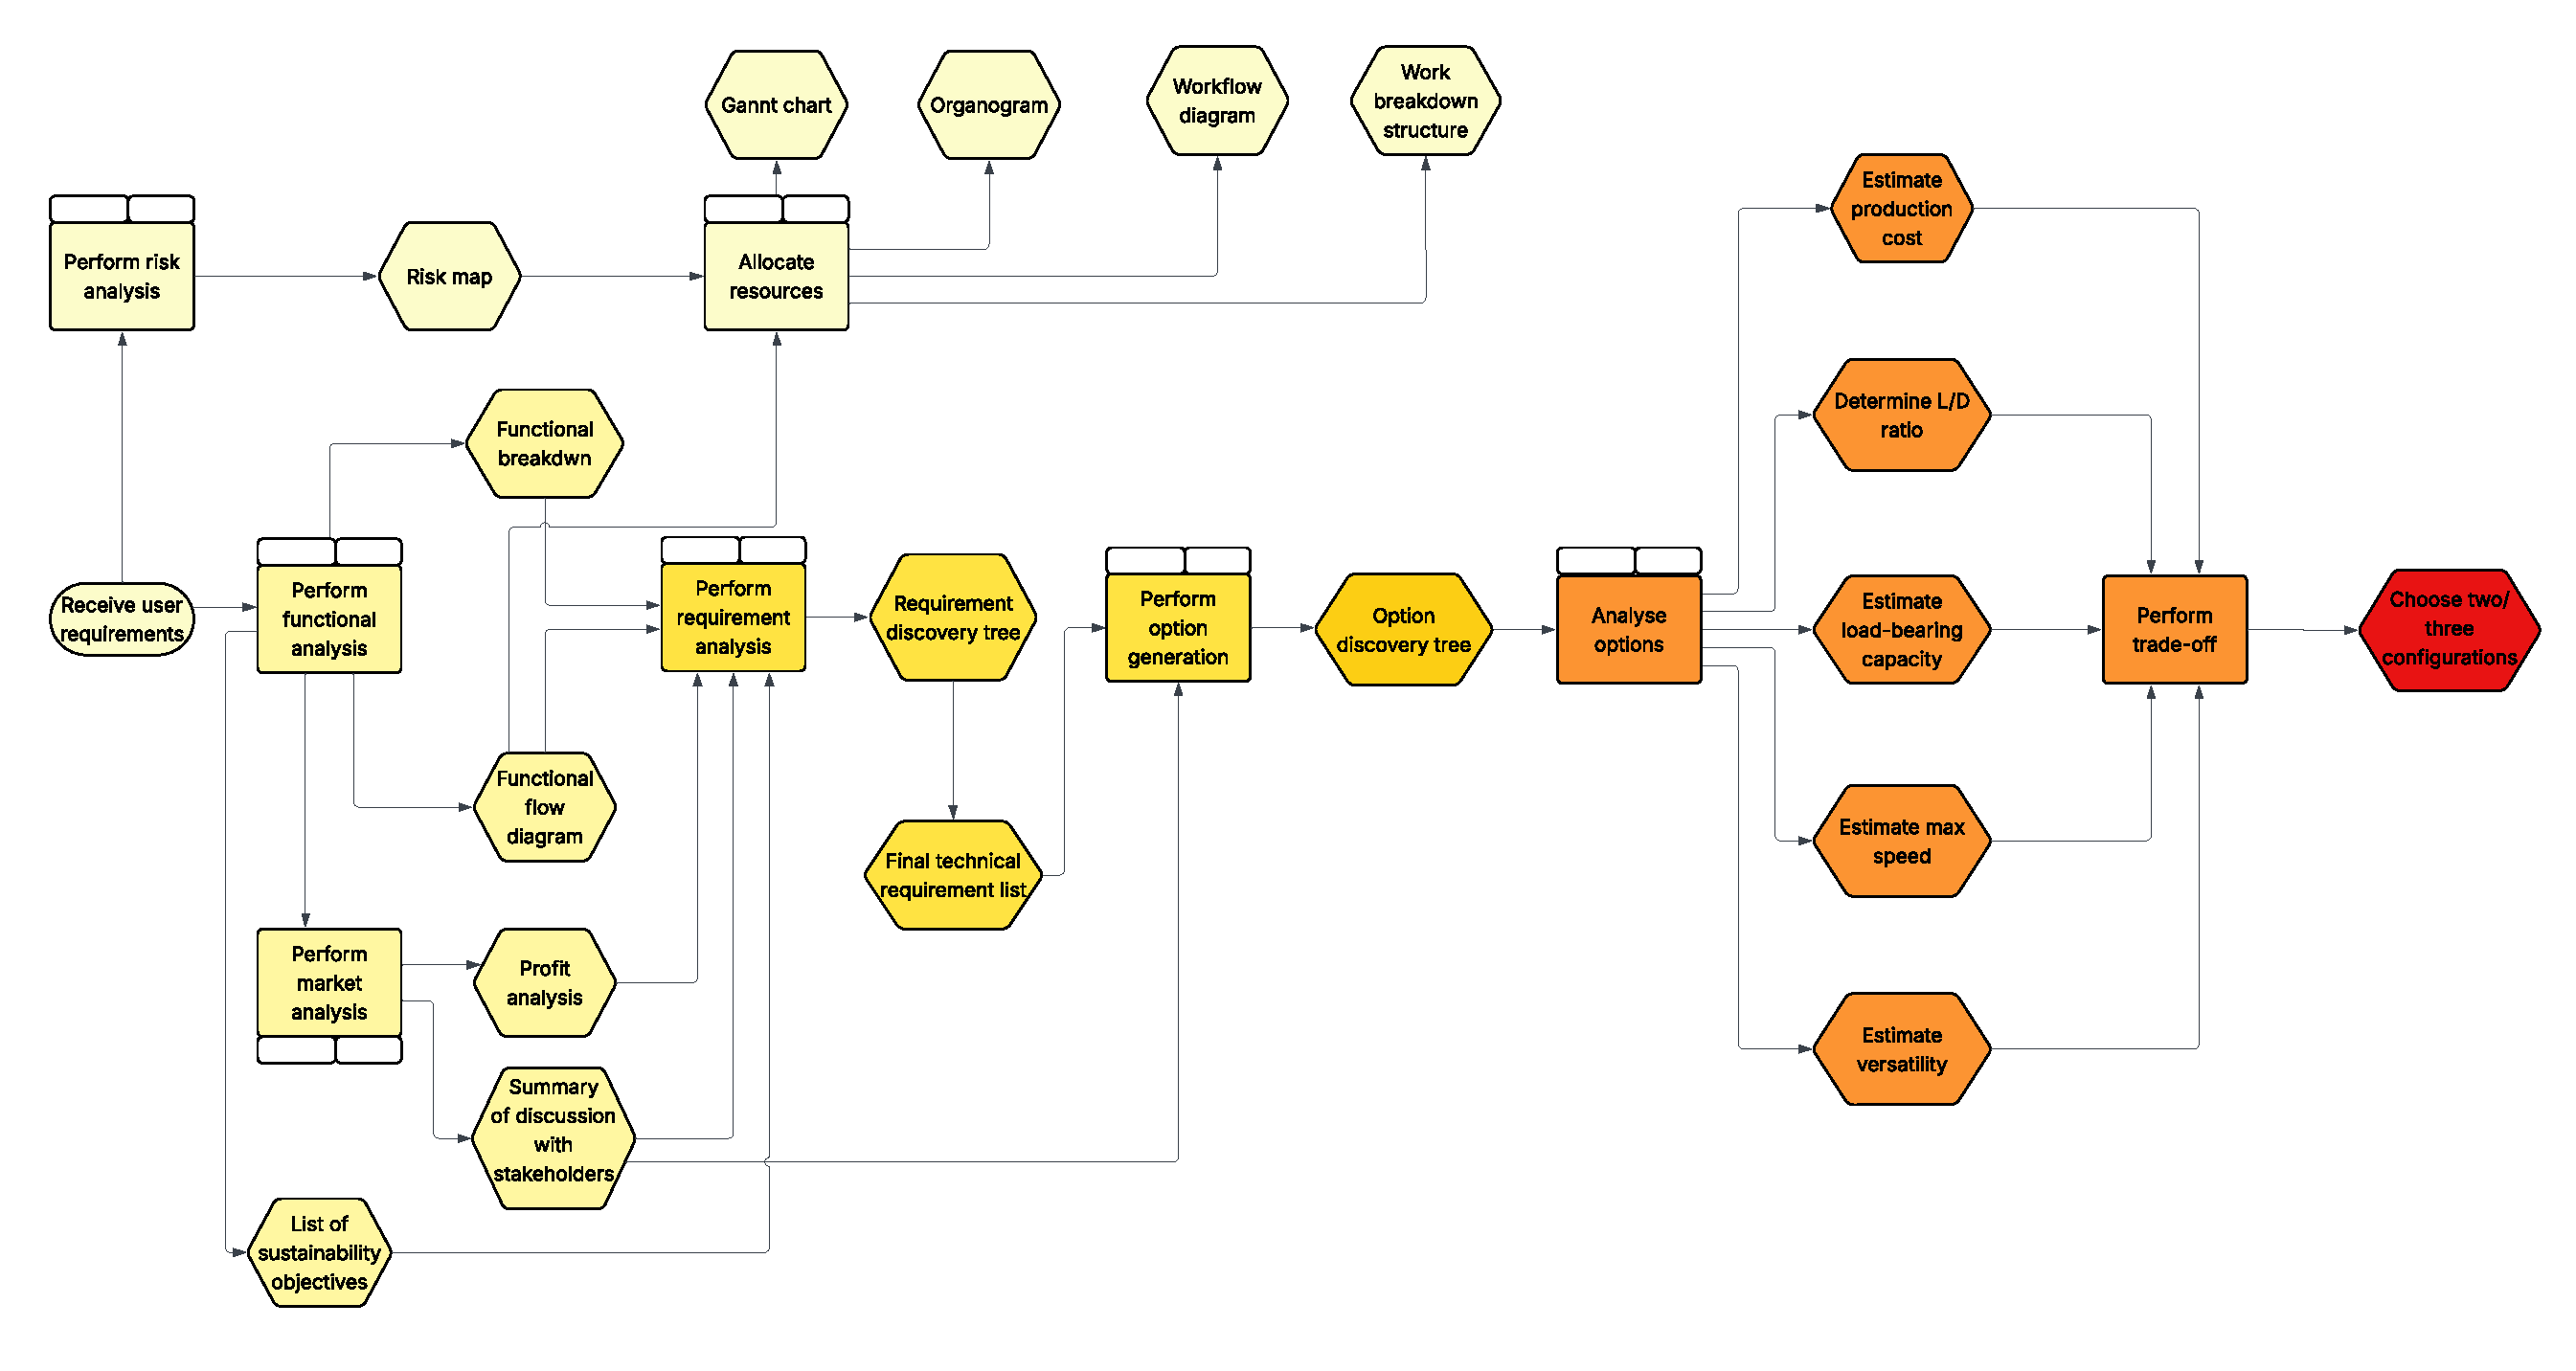
\includegraphics[width=1.4\linewidth, angle=90]{figures/Work-flow baseline.pdf}
    \caption{Work Flow Diagram of the Unmanned Flying Laboratory}
    \label{fig:placeholder}
\end{figure}


\section{Work Breakdown Structure}

A Work Breakdown Structure (WBS) is a hierarchical decomposition of a project into smaller, manageable components. It organizes all the work required to deliver a system into clearly defined elements, typically moving from high-level system functions down to detailed tasks or deliverables. The purpose of a WBS is to improve clarity, assign responsibility, support scheduling and budgeting, and ensure that no critical scope is overlooked.

In the case of the unmanned modular test bed, two key aspects were considered when constructing the WBS: the physical system (air vehicle, payload, control), and the mission purpose (experimental testing, replacing conventional wind tunnels). This separation is important because, unlike a conventional aircraft project, the primary output is not the vehicle itself but the data and experimental capability it provides. Testing is elevated from a verification step to a core operational function. This reflects the idea that the platform acts as a “flying laboratory,” addressing limitations of wind tunnels such as mounting interference, scaling constraints, and inability to test to failure.

\begin{figure}[H]
    \centering
    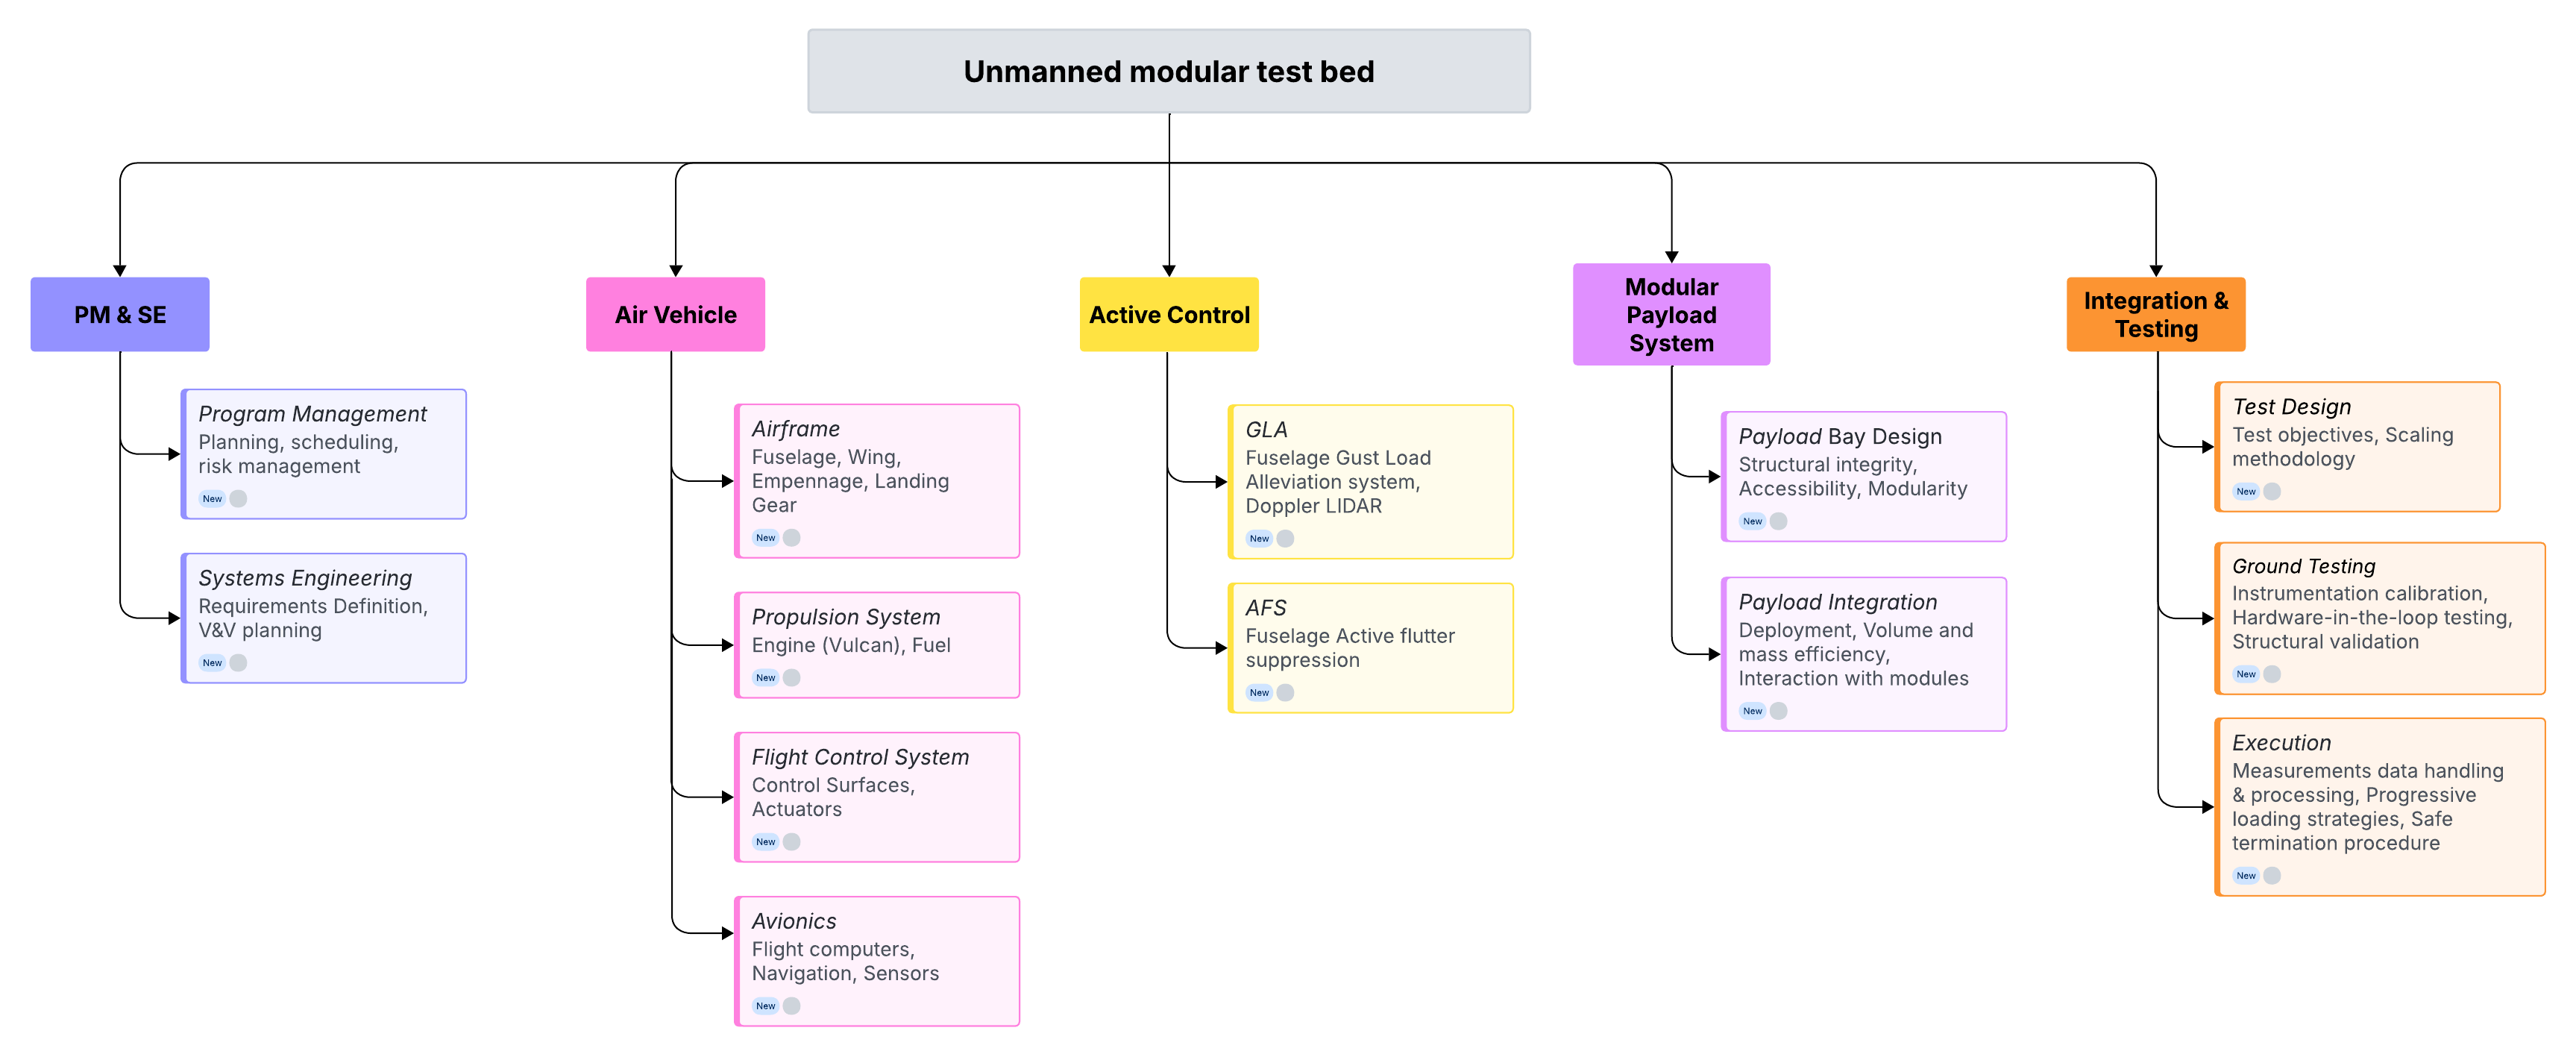
\includegraphics[width=1.1\linewidth]{figures/Work breakdown structure (WBS).png}
    \caption{Work Breakdown Structure of the Unmanned Flying Laboratory}
    \label{fig:placeholder}
\end{figure}



\section{Schedule (Gantt Chart)}
To outline the schedule of the project, all the required deliverables and milestones have been compiled into a Gantt Chart, seen in \autoref{fig:gantt_chart}. It has been decided to work on the large reports: Project Plan, the Baseline Review, the Midterm Review and the Final Review in sequence, completing all other assignments, such as presentation preparation or posters, in parallel.

The Gantt Chart follows a colourblind-safe palette avoiding combinations of red and green. Both full draft and final deadlines are marked (for presentations the final deadline is presenting time) in the chart, and deliverables worked on are specified for every day, holidays excluded.

\begin{figure}
    \centering
    
\includegraphics[width=1.3\linewidth]{figures/GantChart.pdf}
    \caption{The Gantt Chart schedule for the project}
    \label{fig:gantt_chart}
\end{figure}
